% 第 34(2) 题解析：d 为距 c 最近的干涉加强点（TikZ 线稿）
% ad=r1，bd=r2，cd=3l/8；三角形 abc 为等边三角形
\begin{tikzpicture}[font=\small]
  \coordinate (a) at (0,0);
  \coordinate (b) at (3.8,0);
  \coordinate (c) at (1.9,3.291);
  \coordinate (d) at (1.1875,2.0569);   % a 沿 ac 方向 5/8 处
  \draw[dashed] (a) -- (b) -- (c) -- cycle;
  \draw[thick] (a) -- (d);
  \draw[thick] (b) -- (d);
  \draw[dashed] (d) -- (c);
  \fill (a) circle (1.4pt) node[below left] {$a$};
  \fill (b) circle (1.4pt) node[below right] {$b$};
  \fill (c) circle (1.4pt) node[above] {$c$};
  \fill (d) circle (1.4pt) node[left] {$d$};
  \node[left] at (0.60,1.03) {$r_1$};
  \node[right] at (2.55,1.03) {$r_2$};
  \node[right] at (1.95,2.52) {$\dfrac{3l}{8}$};
\end{tikzpicture}
